 \section{Future Recommendations}
	This section contains various recommendations of work that should/ could be completed on the lolly machine. Recommendations have been split into priority levels. High priority items should be completed first followed by medium and finally low. 

    \subsection{High Priority}
    Of all recommendations listed, high priority should be considered first. Each task within this section will impact the overall function of the machine dramatically. High priority recommendations are listed in order of importance.
	
        \subsubsection{New Colour Sensors} 
		
            The colour sensors currently installed on the machine have difficulty in distinguishing between certain colours. This is the biggest hindrance to the completion of the project and is the only thing stopping it from being utilised on open days. My recommendation would be to use a camera based colour detection system capable of determining the colour of an object in hex code format. Hex code ranges can be stored within the \acrshort{plc} with each range corresponding to a different colour. With this setup, there is almost a limitless number of colours that could be stored within the \acrshort{plc}, thus, allowing the user to change the secondary hopper colours ad hoc. This option will require a reasonable about of development and could be suitable as a group project as a part of one of the \acrshort{icse} third or fourth year units.
			
			Alternatively, the colour sensors could be replaced by a newer industrial colour sensor. This option would be faster to implement as the program wouldn't need to be altered. Down sides of this option is price point as industrial colour sensors are relatively expensive.
			
			This task should be completed as soon as possible so the machine is able to be used as intended. 
			
       \subsubsection{New Lollies} 
            Originally, the machine took Allen's Kool Fruits which seemed to work pretty well in regards to size, shape and colour. Unfortunately, Allen's Kool Fruits are now only available in separately packaged plastic bags which for obvious reasons are no good for this application - or the environment! Currently, the lolly machine is full of gum balls. The gum balls are smaller than Allen's Kool Fruits, subsequently, they do not work quite as well. There are two main issues with the gum balls.
			
			\begin{enumerate}
				\item The actuator responsible for transferring the gum balls from the primary hopper into the colour detection shoot will often fail to transfer a gum ball. This is because the gum balls are too small and get wedged in the hopper. Presently, this is being counteracted by isolating the machine and moving the gum balls around with a sterile rod to dislodge stuck gum balls within the hopper.
				\item The proximity sensor that detects the presence of a lolly in the colour detection shoot will often fail to register that a lolly has been dropped. This is because the lollies are too small and sometimes cannot be seen by the proximity sensor. 
			\end{enumerate}
			
			As a corrective action, either find a supplier that sells Allen's Kool Fruits that are not individually wrapped or find a lolly with the same dimensions.
			
			Allen's Kool Fruits have a 19 mm diameter while the gum balls have is approximately 15 mm. This is seen in Figure \ref{fig:gumBallMeas} and \ref{fig:koolFruitMeas}.

           \begin{figure}[H]
        \centering
        \begin{minipage}{0.4\textwidth}
            \centering
            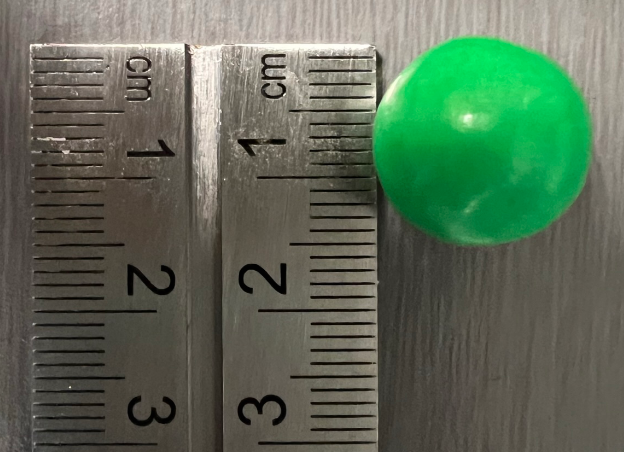
\includegraphics[width = 0.9\textwidth]{2_images/gumBallMeas}
            \caption{Gum balls currently in the lolly machine - too small. }
            \label{fig:gumBallMeas}
        \end{minipage}\hfill
        \begin{minipage}{0.4\textwidth}
            \centering
            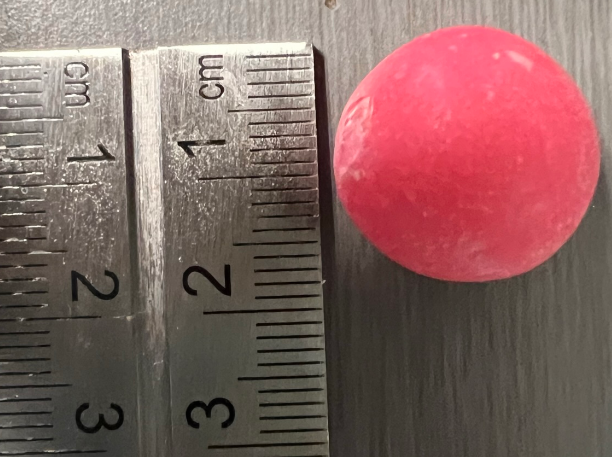
\includegraphics[width = 0.9\textwidth]{2_images/koolFruitMeas}
            \caption{Allen's Kool Fruit that are no longer available - correct size.}
            \label{fig:koolFruitMeas}
        \end{minipage}\hfill            
        \end{figure}  
        
        \subsubsection{Improve Safety Function} 
            Currently, if the \acrshort{estop} is pressed, or an alarm is triggered, the machine will halt operation until the fault has been cleared. This recommendation is to add an isolation valve that feeds all pneumatic control valves. In the event of an alarm, all pneumatic system peripherals will depressurise. This will allow any trapped objects or body parts to be easily removed from critical pinch/ grab points. 
			
			Adding this safety function is important but not critical as all pneumatic actuators are enclosed during normal operation.
			

            

    \subsection{Medium Priority}
    
		Medium priority tasks should be considered after high priority tasks and before low priority tasks
  
        \subsubsection{Bump-less Control} 
            Currently, when you change the control source, i.e., from the \acrshort{hmi} to LabVIEW application, the machine mode will not be transferred. This is a nuisance when one control source is in auto while the other is in manual. Ideally, when the control source is altered the machine mode should be transferred. 

		\subsubsection{Alarm Start Up Delay}
			When the machine starts up it, multiple \acrshort{fto} and \acrshort{ftc} alarms are activated as the valves are often in the `wrong' position during startup. A simple piece of logic should be included to delay the alarm logic from running for the first five seconds. 
            
        \subsubsection{Extra Microcontroller Functionality} 
            Raspberry Pi's and Arduino's have an almost infinite use case. The tasks they are performing, within the confides of this project, is well within the processing capabilities of these devices. This recommendation is open ended and is an invitation to get create.  Use the microcontrollers to do something fun!! As an example, you could link the Raspberry-Pi to a speaker and have it announce the operating mode whenever it is changed. Think outside the box!
        
        \subsubsection{Replace Cables} 
            Due to time restrictions and lack of resources, the cables that link the auto switch terminals to the remote \acrshort{io} are blue which is the same colour as 24 \acrshort{dc} ground cables. This could create confusion later down the track. The cables should be replaced with ones of a different colour.      
 
        \subsubsection{Additional LED functions}
            The traffic light arrangement of \acrshort{led}s on the front panel provide a basic indication to the machine status. Additional machine status information could be displayed by different configurations and flash rates of the \acrshort{led}s. For example, the red \acrshort{led} could flash when the \acrshort{plc} has a system error.
            
    \subsection{Low Priority}
        Low priority recommendations, although may appear somewhat enticing should not be considered until all of the above recommendations have either been completed or ruled out.
        
        \subsubsection{Replace Click PLC} \label{sec:replacePlc}
            Ideally, the lolly machine control system should have been built with hardware of the same make as standardisation allows for a more robust, easier to trouble shoot and in some cases simpler system. At Murdoch, the control hardware of choice seems to be Siemens which is awesome as they make excellent hardware/ software and is prevalent among industry.
            
            This recommendation is to replace the Click \acrshort{plc} with a Siemens \acrshort{plc}. 
            
            Siemens \acrshort{tia} Portal is far superior to Click Programming Software for many reasons. 
            
            One example of one area where this would improve the program is the \acrshort{fto} and \acrshort{ftc} logic. Function blocks (not available in Click Programming Software) would drastically improve development time and also would make troubleshooting much easier.

            I have made a small program within \acrshort{tia} Portal that demonstrates how functions can be utilised to simplify code. This example shows how functions can be used to simplify \acrshort{fto} logic, seen in Figure \ref{fig:ftoFunTia}.
    
            \begin{figure}[H]
                \centering
                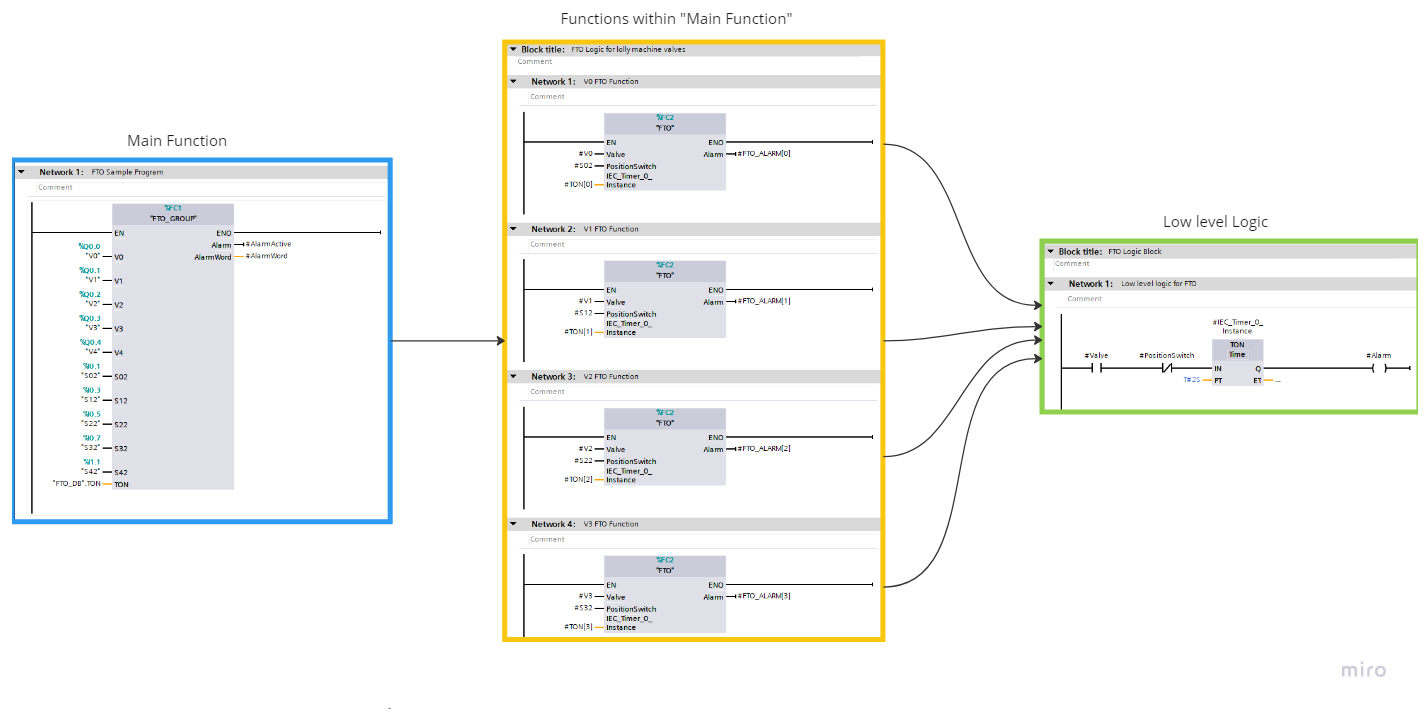
\includegraphics[width = 0.9\textwidth]{2_images/ftoFunTia}
                \caption{An example showing FTO logic using Siemens programming software \acrfull{tia}}
                \label{fig:ftoFunTia}
            \end{figure}
    
        \subsubsection{Add SQL Server to Raspberry Pi}
            A \acrshort{sql} server could be added to the Raspberry Pi. The idea of the server would be to hold process data for trouble shooting a diagnostics. My recommendation would be to use Node-RED to pass the data into the \acrshort{sql} server. This data, could also be used to generate trends. 

\section{Summary}
    The main objective of this project was to overhaul the lolly machine control system to bring it in line with today's technologies while getting it in a functional state for open days. The idea behind the upgrading the control system is to allow future students to continue development on the machine during \acrshort{icse} projects and possibly another thesis. 
    The overhaul of the control system was a great success and everything, from an installation and programming perspective, was achieved. The completion of \acrfull{lmu} has put the machine in an operable state where it is ready for future students to continue development if they so wish. The lolly machine is fully operable and will sort and dispense lollies as a function of the colour detected by the colour sensors. Unfortunately, the existing colour sensors are not able to accurately detect the colour of the lollies 100\% of the time - this means that the machine is not ready for open days. This issue can be easily rectified by installing new colour sensors. 
    Another aspect of this project was to implement multiple user interfaces for the machine. The lolly machine is controllable via multiple \acrshort{hmi}s, namely, a Siemens \acrshort{hmi} a LabVIEW application and  WiFi enabled devices through a service running on a Raspberry Pi. 
    Overall this project has effectively fulfilled the requirements set out in the initial design. The lolly machine is in an operable state ready for future developments and will be ready for use on open days after the colour sensors have been replaced.